
\chapter{L'informazione e il web semantico}

	\section{La torre di Babele del web}
	
		\subsection{Un esempio di problema informativo}
			Con l'espansione del web si sperimentano i primi bot cattura informazione. Uno di questi sistemi creato dal MIT permetteva un acquisto in pochi passi. Una \emph{query} famosa fu "manda una rosa alla mia ragazza", il bot trovò il prodotto desiderato e anche ne trovò un altro che corrispondeva a tutt'altro.
			Lo stesso capitò alla RIA (l'equivalente della SIAE) con un proprio bot che scovò una canzone piratata del cantante Usher ma che in realtà si rivelò una canzone completamente diversa, creata a scopo educativo dal professor Peter Usher.
			Molti investimenti sono stati fatti e ad oggi i bot comprendono meglio le informazioni sfruttando i tipi semantici.
		
		\subsection{Evoluzione}
			Se al posto dell'Html avessimo informazione strutturata potremmo rimuovere le  ambiguità e le macchine potrebbero "capire" le informazioni del web. Uno strumento per fare questo poteva essere l'XML, semplice e flessibile, creato proprio per la necessità di strutturazione dei dati. Purtroppo proprio da questi stessi vantaggi sono nati molti dialetti che rendono impossibile l'\textbf{aggregazione}. L'XML uscì fallimentare dall'\emph{open world} e portò quindi alla necessità di creare un nuovo livello superiore che permettesse l'aggregazione e un nuovo strumento che lo descrivesse: l'RDF. Vediamo i vantaggi rispetto l'XML:
			\begin{itemize}
				\item le informazioni mappano su un modello non ambiguo. In ogni modello RDF si può riconoscere quali bit rappresentano la semantica e quali la sintassi di contorno.
				\item l'RDF è parte del web semantico.
			\end{itemize}
			L'RDF è quello strumento che mancava per rendere possibile l'\textbf{aggregazione} dell'informazione e il ragionamento automatico su di essa.
		
	\section{Il web semantico}
	
		\subsection{Babel Fish: l'RDF}
			Babel Fish è un traduttore istantaneo biologico descritto all'interno del libro \emph{Guida Galattica per gli Autostoppisti} di Douglas Adams. Il modello RDF (\emph{Resource Description Framework}) può certamente interpretare questo ruolo di traduttore dal web che conosciamo a quello semantico come vediamo nella figura ~\ref{fig:LInformazioneEIlWebSemantico-WebSemantico}.
			
			\begin{figure}
				\centering
				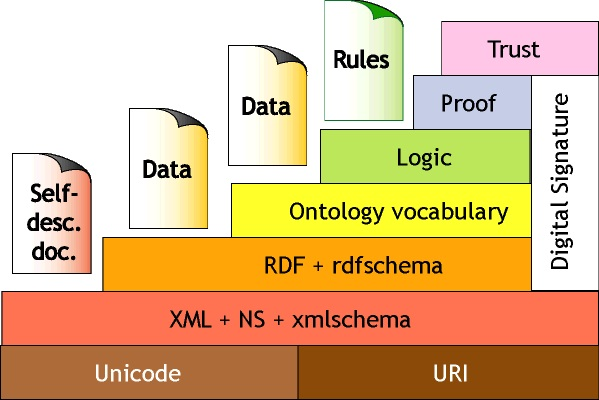
\includegraphics[scale=0.5]{images/LInformazioneEIlWebSemantico-WebSemantico1}
				\caption{Il web semantico - \emph{Layer} che compongono l'informazione}
				\label{fig:LInformazioneEIlWebSemantico-WebSemantico}
			\end{figure}			
			
			\subsubsection{Il modello RDF}
				Il modello RDF è un \emph{framework} comune che descrive metadati, relazioni e concetti garantendo l'interoperabilità tra essi, ossia lo scambio di informazioni senza necessità di traduzioni di linguaggio. Si basa sulla grammatica di base:
				\begin{quote}
					$\langle$ soggetto - predicato - complemento oggetto $\rangle$
				\end{quote}
				Questi tre elementi possono contenere due diversi tipi di dati:
					\begin{itemize}
						\item URI,
						\item Stringhe letterali;
					\end{itemize}
				che compongono la struttura linguistica e logica più semplice. Questa struttura può essere visualizzata come un grafo ~\ref{fig:LInformazioneEIlWebSemantico-RDF1}.
				
				\begin{figure}
				\centering
					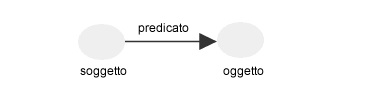
\includegraphics[scale=0.8]{images/LInformazioneEIlWebSemantico-RDF1}
					\caption{Il web semantico - Grammatica di base}
					\label{fig:LInformazioneEIlWebSemantico-RDF1}
				\end{figure}
				
				L'RDF può essere rappresentato in due modi differenti:
				\begin{description}
					\item[dialetto XML] usando la struttura XML per alzare la complessità e arricchire il significato.
					\item[N-triple] usando le triplette "soggetto-predicato-complemento oggetto".
				\end{description}
				Esempio di tripletta della frase \emph{"il cielo è blu"} contenente due stringhe:
				\begin{quote}
				\begin{verbatim}
					<rdf:Description rdf:about='cielo'>
					<v:essere>blu</v:essere>
					</rdf:Description>
				\end{verbatim}
				\end{quote}
				
				L'RDF è un linguaggio separato dal web comune, per integrarlo si è ricorso ad una versione XHTML2: l'RDFa che aggiunge gli attributi \emph{about} (il soggetto) e \emph{property} (il verbo), il contenuto è il complemento oggetto.
				
			
			\subsubsection{Funzionalità e proprietà di RDF}
			
				\begin{description}
					\item[Aggregazione:] l'unione di due grafi di conoscenza è un grafo creato tramite collegamenti automatici dei nomi del web (URI). Questa è la proprietà più importante e che decreta il successo di RDF rispetto ai dialetti XML. 
					\item[Contenitori:] concetti logici di AND e OR.
					\item[Variabili:] oggetti logici non specificati.
					\item[Monotonicità:] preso un grafo, se l'informazione espressa in esso è vera allora tutti i sotto-grafi sono veri.
					\item[Reificazione:] garantisce la monotonicità, riduce ad un oggetto (\emph{"cosifica"} cit.) una asserzione. Per esempio nella frase \emph{"Gromit dice che 'la luna è di formaggio'"}, la frase nel sottolivello \emph{"la luna è di formaggio"} è in realtà un'altra frase che grazie al processo di reificazione diventa un oggetto, per cui, anche se non sappiamo sia vero ciò non influisce nella veridicità della prima frase. Grazie a ciò abbiamo anche una diversificazione di livelli.
				\end{description}
				
				Gli oggetti devono essere anche classificati garantendo un costo computazionale minimo. Abbiamo bisogno di un \textbf{sistema di classificazione dell'informazione}: un'ontologia che contenga tipi semantici. Mentre i \textbf{tipi} danno il formato sintattico dell'oggetto, i \textbf{tipi semantici} gli danno il significato astraendo la rappresentazione sintattica.
				
			\subsubsection{I tipi semantici}
				Abbiamo visto con il caso \emph{"Usher vs Peter Usher"} che nel web mancano i tipi semantici. I tipi semantici possono essere astratti come classi. Un insieme di classi forma un'ontologia. Un'ontologia è costituita da:
				\begin{description}
					\item[Etichette:] rappresentanti caratteristiche informative (possono essere più di una per oggetto).
					\item[Struttura:] rappresentante la gerarchia di tutte le classi. Più una struttura è ricca e più l'ontologia mi permette di espandere le cose e la comprensione di esse. È grazie alla struttura che è possibile fare \textbf{controlli di integrità semantica} e \textbf{ragionamenti}.
				\end{description}
				
			\subsubsection{Caratteristiche di RDF Schema}
				L'RDF offre uno schema con una struttura informativa fatta di:
				\begin{itemize}
					\item \emph{Class};
					\item \emph{subClassOf};
					\item \emph{individual}.
				\end{itemize}
				Questo per gli oggetti mentre per i verbi abbiamo a disposizione:
				\begin{itemize}
					\item \emph{Property}; (la relazione, il verbo)
					\item \emph{subPropertyOf};
					\item \emph{Domain};
					\item \emph{range}. (dove la proprietà è applicata)
				\end{itemize}
				Grazie all'RDF Schema, quindi, possiamo \textbf{categorizzare l'informazione}.

			\subsubsection{Oltre l'RDF Schema}
				Abbiamo fissato delle regole semantiche ma siamo ancora al livello base delle ontologie (stato tassonomie). Si può fare molto di più: l'RDF permette l'aggregazione automatica attraverso l'URI. Ma gli URI presentano problemi di ambiguità.
			
		\subsection{L'architettura del web (Tim Berners-Lee)}
			Tim Berners-Lee prevedeva già questo alla nascita del web e infatti il web è nato seguendo questi assiomi:
			\begin{itemize}
				\item [0a)] A qualsiasi risorsa dovunque sia, essa può avere un nome. (\emph{assioma di universalità})
				\item [0b)] Ogni cosa di significato dovrebbe avere un URI. (\emph{assioma di universalità 2})
				\item [1)] Non importa a chi o dove specifichi un URI, ma che abbia sempre lo stesso significato. (\emph{global scope})
			\end{itemize}
			
			\subsubsection{Dare un nome ad ogni cosa: il problema degli URI}
				Trovare un nome (web) non è banale:
				\begin{description}
					\item[URI \emph{variant problem}:] esistono molte varianti per lo stesso concetto.
					\item[URI \emph{variant law}:] l'utilità decresce esponenzialmente con il numero di varianti (legge della varianza degli URI). Più un nome ha diversi significati più questo perde valore.
					\item[URI \emph{variant size}:] un URI può acquisire diversi significati in base al dominio di interesse. "Problema \emph{big red barn}" cit. (se un bambino indica una mucca illustrata in un libro, ciò che indica è "una mucca" o "un libro"? Esistono livelli diversi).
				\end{description}				
			
			\subsubsection{La soluzione}
				La soluzione a questo inghippo è aggiungere più informazione. Abbiamo bisogno di maggiore informazione, un nuovo \emph{layer}: lo strato ontologico e un nuovo linguaggio.
		
		\subsection{Strato ontologico: OWL}
			Il supporto di base fornito da RDF Schema è stato quindi esteso con lo strato ontologico. Questo strato è descritto attraverso il linguaggio OWL (\emph{Web Ontology Language}) che si occupa di collegare e relazionare i vocaboli dando ad ognuno il proprio dominio d'interesse (la propria ontologia appunto).
		
			\subsubsection{Caratteristiche e proprietà di OWL}
				In OWL si può parlare dell'(in)uguaglianza degli oggetti. Per fare questo definisce le funzionalità:
					\begin{itemize}
						\item equivalentClass: per capire se due classi di vocabolari identificano la stessa.
						\item equivalentProperty: per capire se due \emph{property} (verbi) hanno stesso significato.
						\item sameIndividualAs
						\item differentFrom
						\item allDifferent
					\end{itemize}
					
				Grazie a queste funzionalità si riesce a risolvere il problema dei nomi e a mappare ontologie diverse sotto lo stesso grafo. Altre funzionalità offerte da OWL:
				
					\begin{itemize}
						\item inverseOf: collegare due proprietà per complementarietà.
						\item transitiveProperty: capire se una proprietà è transitiva.
						\item simmetricProperty (l'amicizia su Facebook è simmetrica).
						\item inverseFunctionalProperty: specificare se un certo verbo è funzionale o no (dato un oggetto c'è un solo complemento oggetto associato).
					\end{itemize}
					
				Sono inoltre possibili utilizzare restrizioni sulle proprietà delle classi:
				\begin{itemize}
					\item allValueFrom ($\forall$);
					\item someValueFrom ($\exists$);
					\item minCardinality
					\item maxCardinality
					\item cardinality
				\end{itemize}
				
			\subsubsection{Il problema: ragionarci}
				Abbiamo tutte queste informazioni su cui ragionarci. Ma come? Purtroppo quando si passa ad un ragionamento ad alto livello la logica diventa indecidibile. Per descrivere espressioni ad alto livello sulle macchine è necessaria una traduzione a basso livello poiché la logica di prim'ordine, che fa uso dei costrutti logici $\exists$ e $\forall$, non è decidibile (la macchina non sa creare un programma che termini sempre). È il motivo per cui non abbiamo ancora linguaggi di programmazione ad alto livello che seguono una scrittura più vicina al nostro linguaggio.
			
		\subsection{SPARQL}
			Abbiamo bisogno di un linguaggio che permetta una comunicazione di alto livello (relazionale) e che si occupi lui di definire la parte di basso livello. Un linguaggio simile funzionante è SQL in cui definisce tabelle e relazioni. Per permettere di garantire la terminazione del programma, SQL è vincolati da alcuni limiti. La stessa cosa è stata applicata al web semantico sostituendo le relazioni tra tabelle con relazioni in un grafo generico. Nasce così SPARQL (SPARQL \emph{Protocol And RDF Query Language}), il linguaggio per permettere le \emph{query} nel web semantico seguendo le scelte di design di SQL.
		
			\subsubsection{Modellazione con SPARQL}		
				Il fattore principale di SPARQL è il \emph{pattern matching} tra triplette nella struttura a grafo. 
				
				La struttura di una \emph{query} SPARQL è:
				\begin{quote}
				\begin{verbatim}
					PREFIX ...
					SELECT ...
					FROM ...
					WHERE ( ...
								)
					ORDER BY ...					
				\end{verbatim}					
				\end{quote}					
				
		\subsection{Vocabolari ontologici}
		
				\subsubsection{DC: Dublin Core}
					Il Dublin Core è uno dei primi tentativi di strutturare il web in maniera semantica, descrivendo le pagine web URI. Definisce le proprietà di base fondamentali e essenziali che modellano l'intera struttura dei dati semantici. Queste proprietà di base individuate sono 15 che elenchiamo per completezza:
					\begin{enumerate}
						\item \emph{Title}
						\item \emph{Creator}
						\item \emph{Subject}
						\item \emph{Description}
						\item \emph{Publisher}
						\item \emph{Contributor}
						\item \emph{Date}
						\item \emph{Type}
						\item \emph{Format}
						\item \emph{Identifier}
						\item \emph{Source}
						\item \emph{Language}
						\item \emph{Relation}
						\item \emph{Coverage}
						\item \emph{Rights}
					\end{enumerate}
				Un insieme compatto che mi permette di definire una pagina web in triplette che compongono un grafico della conoscenza su cui è possibile effettuare delle \emph{query}.
				Per esempio, usando i \emph{tag meta} è possibile tramite la \emph{keyword} '\emph{DC}' mettere a disposizione queste triplette direttamente nel web in modo che bot intelligenti ricavino informazioni utili.
				\begin{quote}
				\begin{verbatim}
					<meta name="DC.title" content="How to use DC" />
					<meta name="DC.creator" ... />
					...
				\end{verbatim}
				\end{quote}
				
				\subsubsection{FOAF: Friend Of A Friend}
					Altro vocabolario per altro usato da Google. Nato per la socialità e non le pagine web. Definisce le proprietà base di una persona. Per la class Person per esempio abbiamo:
					\begin{itemize}
						\item \emph{Name} (pagina web)
						\item \emph{Title} (pagina web)
						\item \emph{Firstname}
						\item[] \dots
						\item \emph{myerBriggs} (uno dei 16 tipi di personalità)
						\item[] \dots
					\end{itemize}
					
					Ad esempio:
					\begin{quote}
					\begin{verbatim}
						<foaf:Person>
						<foaf:name>Massimo Marchiori</foaf:name>
						<foaf:mbox rdf:resource=mailto:massimo@w3.org />
						</foaf:Person>
					\end{verbatim}
					\end{quote}	
					È inoltre possibile esprimere il concetto di 'amicizia' con la relazione \verb|foaf:Knows|. Qui è possibile osservare la difficoltà della scrittura ad annidamento di XML a differenza delle semplici triplette.
					
		\subsection{Un esempio}
			 PlanetRDF è un esempio di base di dati costruita sul web semantico. Tramite le informazioni semantiche con i vocabolari descritti sopra in ogni pagina è stato creato un grafo della conoscenza su cui era possibile effettuare \emph{query}.
		 
		 \subsection{Ancora SPARQL}
		 	Preso il grafo della conoscenza, una base di dati, con SPARQL è possibile eseguire la propria \emph{query}. Per esempio vogliamo prendere l'indirizzo del blog di 'Mario Rossi' dal database planetRDF.
		 	\begin{quote}
		 	\begin{verbatim}
		 		PREFIX foaf:<http://xmlns.com/foaf/0.1/>
		 		SELECT ?url
		 		FROM <http://planetRDF.com />
		 		WHERE (
		 				?someone foaf:name "Mario Rossi"
		 				?someone foaf:webblog ?url		)
		 	\end{verbatim}
			\end{quote}
			
			\subsubsection{Extra SPARQL}
				Una caratteristica di SPARQL interessante è la possibilità di ricerca con dati opzionali, ossia nulli o assenti. Nel web semantico è facile avere informazioni parziali per questo in SPARQL è stato previsto l'operatore \verb|OPTIONAL|. Ad esempio:
				\begin{quote}
				\begin{verbatim}
					PREFIX foaf:<http://xmlns.com/foaf/0.1/>
					SELECT ?name ?picture
					FROM <http://planetRDF.com />
					WHERE (
							?someone foaf:name ?name
							OPTIONAL{
									?picture foaf:picture
									}
					)
				\end{verbatim}
				\end{quote}
				La \emph{query} cerca il nome e la foto di qualcuno, grazie all'uso di \verb|OPTIONAL|, nel caso in cui qualcuno non abbia caricato la propria foto questa \emph{query} non darà errore.
		
		\subsection{Un problema di complessità}
			SPARQL è decidibile come SQL? È efficiente?  Qual è la sua complessità?
			La \textbf{gerarchia dei problemi}, individuata dagli studi sulla complessità, è:
			\[
				NL \subset P \subset NP \subset PSPACE \subset EXPTIME \subset EXPSPACE
			\]
			
			\begin{figure} [h]
				\centering
				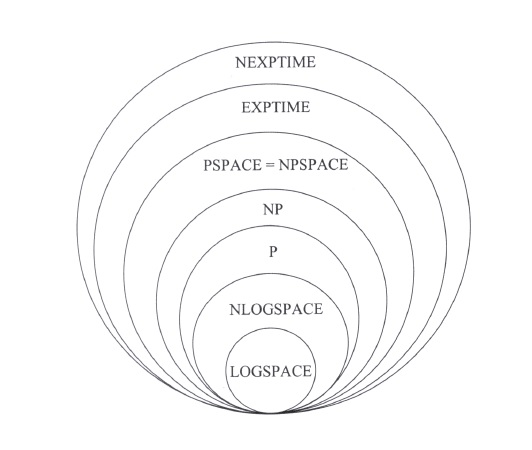
\includegraphics[scale=1]{images/LInformazioneEIlWebSemantico-Complessita}
				\caption{L'informazione e il web semantico - Gerarchia dei problemi}
				\label{LInformazioneEIlWebSemantico-Complessita}
			\end{figure}
			
			Nel design del linguaggio SPARQL si sono seguite le scelte di SQL, per cui è decidibile (ovvero termina) ma ha una complessità $PSPACE$ (spazio polinomiale a rischio).
			

			\subsubsection{La soluzione di OWL}
				Con OWL invece si è optato per mantenere:
				\begin{itemize}
					\item l'\textbf{espressività}, cioè avere una logica espressiva ma complessa da gestire;
					\item la \textbf{computabilità}, cioè avere una logica decidibile ma limitata.
				\end{itemize}
				Per garantirle entrambe, si sono creati dei sottoinsiemi di OWL:
				\begin{description}
					\item[OWL \emph{lite}:] decidibile con uso della logica SHIFT.
					\item[OWL \emph{DL}:] decidibile con logiche descrittive SHOIN.
					\item[OWL \emph{full}:] indecidibile ma sfrutta le logiche più avanzate.
				\end{description}
				
			\subsubsection{Complessità e statistica}	
				La complessità della logica SHIFT è $EXPTIME$ (\emph{query} a tempo esponenziale) mentre per SHOIN è $NEXPTIME$ (tempo esponenziale non deterministico) mentre per OWL \emph{full} non possiamo dire che termini sempre. Viene da pensare per quale assurdo motivo usare strumenti con questa complessità in zone esponenziale ma la complessità è una statistica. È molto più rilevante la statistica su dati non casuali e sopratutto non su qualsiasi combinazione esistente. Per esempio la media ricavata degli input più d'interesse.
					
				\paragraph*{Complessità e pratica} Nell'uso pratico anche se la complessità è in tempo esponenziale la maggior parte delle \emph{query} rientra in complessità molto più basse. Per esempio molta dell'algoritmica di Google sta in $EXPTIME$ ma le \emph{query} più frequenti stanno molto al di sotto. Solo alcune \emph{query} sono esponenziali e il problema è risolto attraverso interruzioni di esse con timer. 
				In SPARQL che è in $PSPACE$ soltanto togliendo la \emph{keyword} \verb|OPTIONAL| scendiamo nella complessità (assoluta) in $co-NP$. A livello statistico molta informazione all'interno del web non è casuale ma segue un ordine e non rientra nella logica indecidibile ma in logiche studiate: OWL DL ha logica ALC e OWL \emph{Lite} AL che corrispondono rispettivamente a complessità PSPACE e P.				
		
	\section{Il web semantico diventa Linked Data}
		Passiamo all'uso del web semantico che per una scelta di \emph{marketing} è stato definito come \textbf{\emph{Linked Data}}.
		
		\subsection{Classificazione LOD}
			I LOD sono i tipi di \emph{Linked Data Open}, ossia disponibili a tutti gratuitamente. Sono classificati in una scala da 1 a 5 stelle.
			\begin{description}
				\item[$\bigstar$] dati sul web liberi (\emph{open}).
				\item[$\bigstar \bigstar$] dati sul web liberi con formato strutturato ovvero \emph{machine readable}.
				\item[$\bigstar \bigstar \bigstar$] dati sul web liberi con formato dati non proprietario (non necessariamente con RDF).
				\item[$\bigstar \bigstar \bigstar \bigstar$] dati sul web liberi con formato \emph{semantic web}.
				\item[$\bigstar \bigstar \bigstar \bigstar \bigstar$] dati sul web liberi con formato \emph{semantic web} collegati ad altri per darli un contesto.
			\end{description}
			
			\begin{figure}
				\centering
				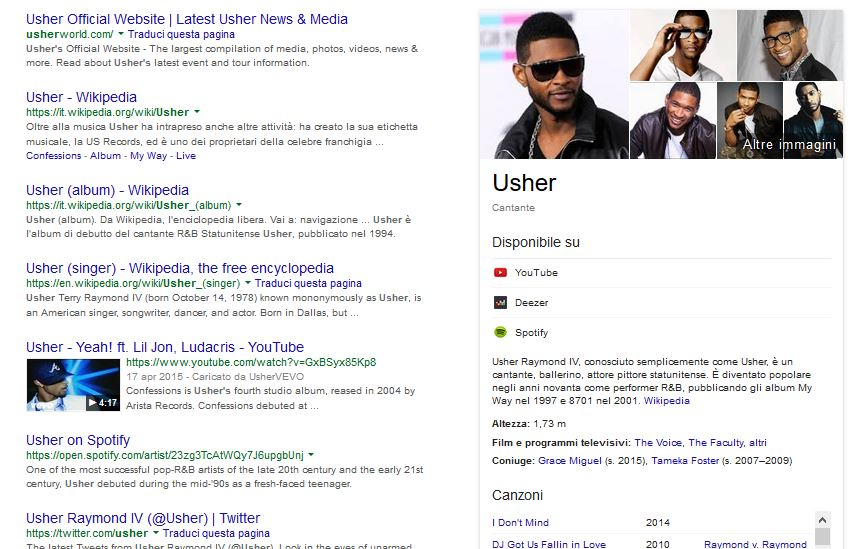
\includegraphics[width=\textwidth]{images/LInformazioneEIlWebSemantico-IlCasoUsher}
				\caption{Il web semantico - Informazione strutturata (sulla destra) raccolta tramite \emph{lifting}}
				\label{fig:LInformazioneEIlWebSemantico-IlCasoUsher}
			\end{figure}
			
		\subsection{Lifting \& lowering}
			\emph{Lifting} \& \emph{lowering} corrispondono, rispettivamente, al passaggio dal mondo a 3 stelle al mondo semantico di 4 e 5 stelle e viceversa.
			Esempi di strumenti di \emph{lifting} sono:
			\begin{itemize}
				\item DR2Q: trasforma il linguaggio SQL in RDF.
				\item Triplify: \emph{plug-in} leggero che crea una struttura semantica da database relazionali.
				\item Openlink 'virtuoso': server universale che permette la relazione tra SQL, XML e RDF.
			\end{itemize}
			Per \emph{lifting} dal formato più basso:
			\begin{itemize}
				\item Open Calais: da un significato al testo e all'informazione pura.
				\item Spotlight.
				\item Alchemy.
			\end{itemize}
			Un esempio di quanto potenziale offrono questi strumenti ce lo fornisce il sito \href{http://www.wikido.com/}{www.wikido.com}. Questo sito preleva da un insieme di siti selezionati informazione che con Open Calais viene trasformata in informazione di alto livello ottenendo dati strutturati.
			Lo stesso fa Google con particolari \emph{query} (vedi figura ~\ref{fig:LInformazioneEIlWebSemantico-IlCasoUsher}).
			
		
		\subsection{Connettere le informazioni: il Mash Up}
			Abbiamo visto le immense potenzialità che derivano dal \emph{lifting} dei dati, ma come è possibile fare questo? Di seguito spieghiamo un tipo di algoritmo adottato da Google che permette questa "magia".
			
			\paragraph*{Il problema:}  Dati due grafi di conoscenza dobbiamo collegarli (se sono collegabili). Per fare questo ci serve una funzione che dati due oggetti web in input, abbia in output un valore di similitudine.
			Immaginando una funzione $simil(x,y)$ posso ottenere un livello di similitudine, se ottengo entro una certa soglia relaziono $x$ con $y$. Con una tecnica di \emph{brute force} otterrei una complessità pari a:
			\[
				O(|G_1| \cdot |G_2|) 
			\]
			perché sto elaborando i \emph{BIG DATA}.
			
			Una tecnica più efficace sfrutta la \textbf{distanza di Levenshtein} che misura la distanza tra due stringhe. Ad esempio una stringa con un carattere diverso da un altra ha distanza 1. È grazie all'uso di esse che Google o qualsiasi altro motore di ricerca mette a disposizione una correzione della \emph{query} inserita dall'utente, ricerche correlate o suggerimenti.
			
			Andando più fini, possiamo sfruttare le proprietà delle distanze:
			\begin{itemize}
				\item $d(x,y)\ge 0$
				\item $d(x,y)=0 \Leftrightarrow x=y$
				\item $d(x,y)=d(y,x)$
				\item $d(x,y) \le d(x,z)+d(z,y)$ (limite superiore)
			\end{itemize}
			Ci interessa la distanza tra due oggetti e con l'ultima proprietà posso ottenere un'approssimazione:
			\begin{align}
				d(x,z) &\le d(x,y)+d(y,z) \\
				d(x,z)-d(y,z) &\le d(x,y) \quad \quad \text{(limite inferiore)}
			\end{align}
			Da cui:
			\[
				d(x,z)-d(y,z) \le d(x,y) \le d(x,z) + d(z,y)
			\]
			Così, invece di calcolare $d(x,y)$ calcoliamo un range d'approssimazione se sappiamo la distanza da un punto $z$ (che descrive geometricamente una stringa). Per sfruttare ciò quindi abbiamo necessità di calcolare la distanza dai punti $z$ (\emph{exemplar}). Con più punti \emph{exemplar} più avremo un range preciso al costo di più calcoli. Fissiamo quindi un numero di punti \emph{exemplar} e calcoliamo solo in essi la distanza riducendo il numero di calcoli.
			Per diminuire al minimo il numero di punti \emph{exemplar} e far sì che questi diano un range d'approssimazione accettabile dobbiamo prendere punti distribuiti equamente. 
			Iniziamo scegliendo un punto e calcoliamo tutte le distanze tra lui e gli altri punti. Dopodiché scegliamo il punto con la distanza maggiore calcolata e ripetiamo lo stesso procedimento in modo da ottenere sempre i punti il più distante possibile.
			Decisi quanti sceglierne otteniamo uno spazio informativo diviso in aree associabili ai punti focali. In ogni zona posso avere delle \textbf{classifiche} dei punti più vicini rispetto ai punti focali, per cui, tornando al problema iniziale, utilizziamo questa tecnica per ottenere i valori di similitudine fissando sempre una soglia e utilizzando i range di approssimazione. Il calcolo:
			\[
				simil(x,y) \le \text{soglia}
			\]
			Con questa tecnica diviene:
			\[
				\text{Se} d(x,z) - d(y,z) > \text{soglia} \Rightarrow d(x,y)>\text{soglia}
			\]
			Con un'unica operazione (una differenza) sappiamo già quale punti scartare poiché le distanze le abbiamo già calcolate.
			
			Ad esempio:
				Prendiamo un \emph{exemplar} del grafo $G_1$ e scegliamo un elemento di $G_2$: $y$, non appena:
				\begin{align}
					simil(x,exemplar)-simil(y,exemplar)&>soglia \\
					\Rightarrow \quad simil(x,y)&>soglia
				\end{align}
				e scartiamo $y$. Inoltre anche per ogni altro $x$ della partizione (sotto la classifica della zona precalcolata) varrà la stessa cosa sempre (la soglia sarà ancora maggiore) per cui rimuoviamo il calcolo per tutti gli altri punti al di sotto della classifica, con un'operazione soltanto.	
				Solo per le coppie non scartate da questa tecnica facciamo $simil(x,y)>soglia$.
		
			\subsubsection{Quanti punti e la complessità}
				Scegliere il numero di punti \emph{exemplar} si rivela il vero problema. Si è visto sperimentalmente che il numero ottimale di punti è la radice quadrata della  dimensione dei dati (grafo più grande). La complessità quindi risulta:
				\[
					O(|E| \cdot |G_1|) + O(|G_1| \cdot |G_2|) = O((|E| + |G_2|) \cdot |G1|)
				\]
				Siamo partiti da con una complessità pari a $O(|G_1|\cdot|G_2|)$ con la tecnica \emph{brute force} e siamo arrivati a $O((|E| + |G_2|) \cdot |G1|)$. Abbiamo ottenuto un algoritmo peggiore ma nella pratica si è rivelato performante portando ad avere anche un risparmio di costo computazionale del 95\% rispetto al \emph{brute force}.
			
			\subsubsection{Esporre i dati}
				Per esporre i dati nel web abbiamo diversi modi. Uno può essere quello di mostrare i dati come file sotto un URI, ma questo è poco pratico. Nella pratica si preferisce ricorrere a interfacce con cui fare \emph{query} usando SPARQL, offrendo in questo modo un servizio web molto potente e flessibile. Questi \emph{query} fatte attraverso indirizzo web con classici \emph{"urlencoding"} e passaggio parametri con GET HTTP sono chiamate \textbf{\emph{endpoint}}. Un esempio di SPARQL \emph{endpoint}:
				\begin{quote}
				\begin{verbatim}
					PREFIX dc <http://purl.org/dc/elements/1.1/>
					SELECT ?book ?who
					WHERE ( ?book dc:creator ?who )
				\end{verbatim}
				\end{quote}
				Un esempio concreto di un tale servizio è \href{http://wiki.dbpedia.org/}{dbpedia.com} da cui è possibile effettuare \emph{query} SPARQL e ottenere pagine come questa: tutta la conoscenza di \href{http://dbpedia.org/page/Albert_Einstein}{Albert Einstain} in una pagina.
				Le ontologie principali sono date da \href{https://schema.org/}{schema.org}. Un altro sito interessante è \href{http://www.visualdataweb.org/relfinder.php}{www.visualdatamedia.org}, il quale mette a disposizione un servizio che permette di navigare il grafo delle conoscenza sulle parole date. 
					
					
					